% Espectro de atención: descomposición espectral del operador de atención
% Muestra eigenvalores decrecientes y eigenfunciones asociadas
% Compilar con: pdflatex attention_spectrum.tex
\documentclass[tikz,border=10pt]{standalone}
\usepackage{tikz}
\usepackage{amsmath,amssymb}
\usetikzlibrary{arrows.meta, positioning, calc, decorations.pathreplacing}

% GDL color palette
\definecolor{gdlblue}{RGB}{41, 98, 168}
\definecolor{gdlred}{RGB}{191, 49, 49}
\definecolor{gdlgreen}{RGB}{30, 130, 76}
\definecolor{gdlorange}{RGB}{217, 130, 30}
\definecolor{gdlpurple}{RGB}{118, 56, 138}
\definecolor{gdlgray}{RGB}{140, 140, 140}
\definecolor{gdlyellow}{RGB}{190, 140, 10}

\begin{document}
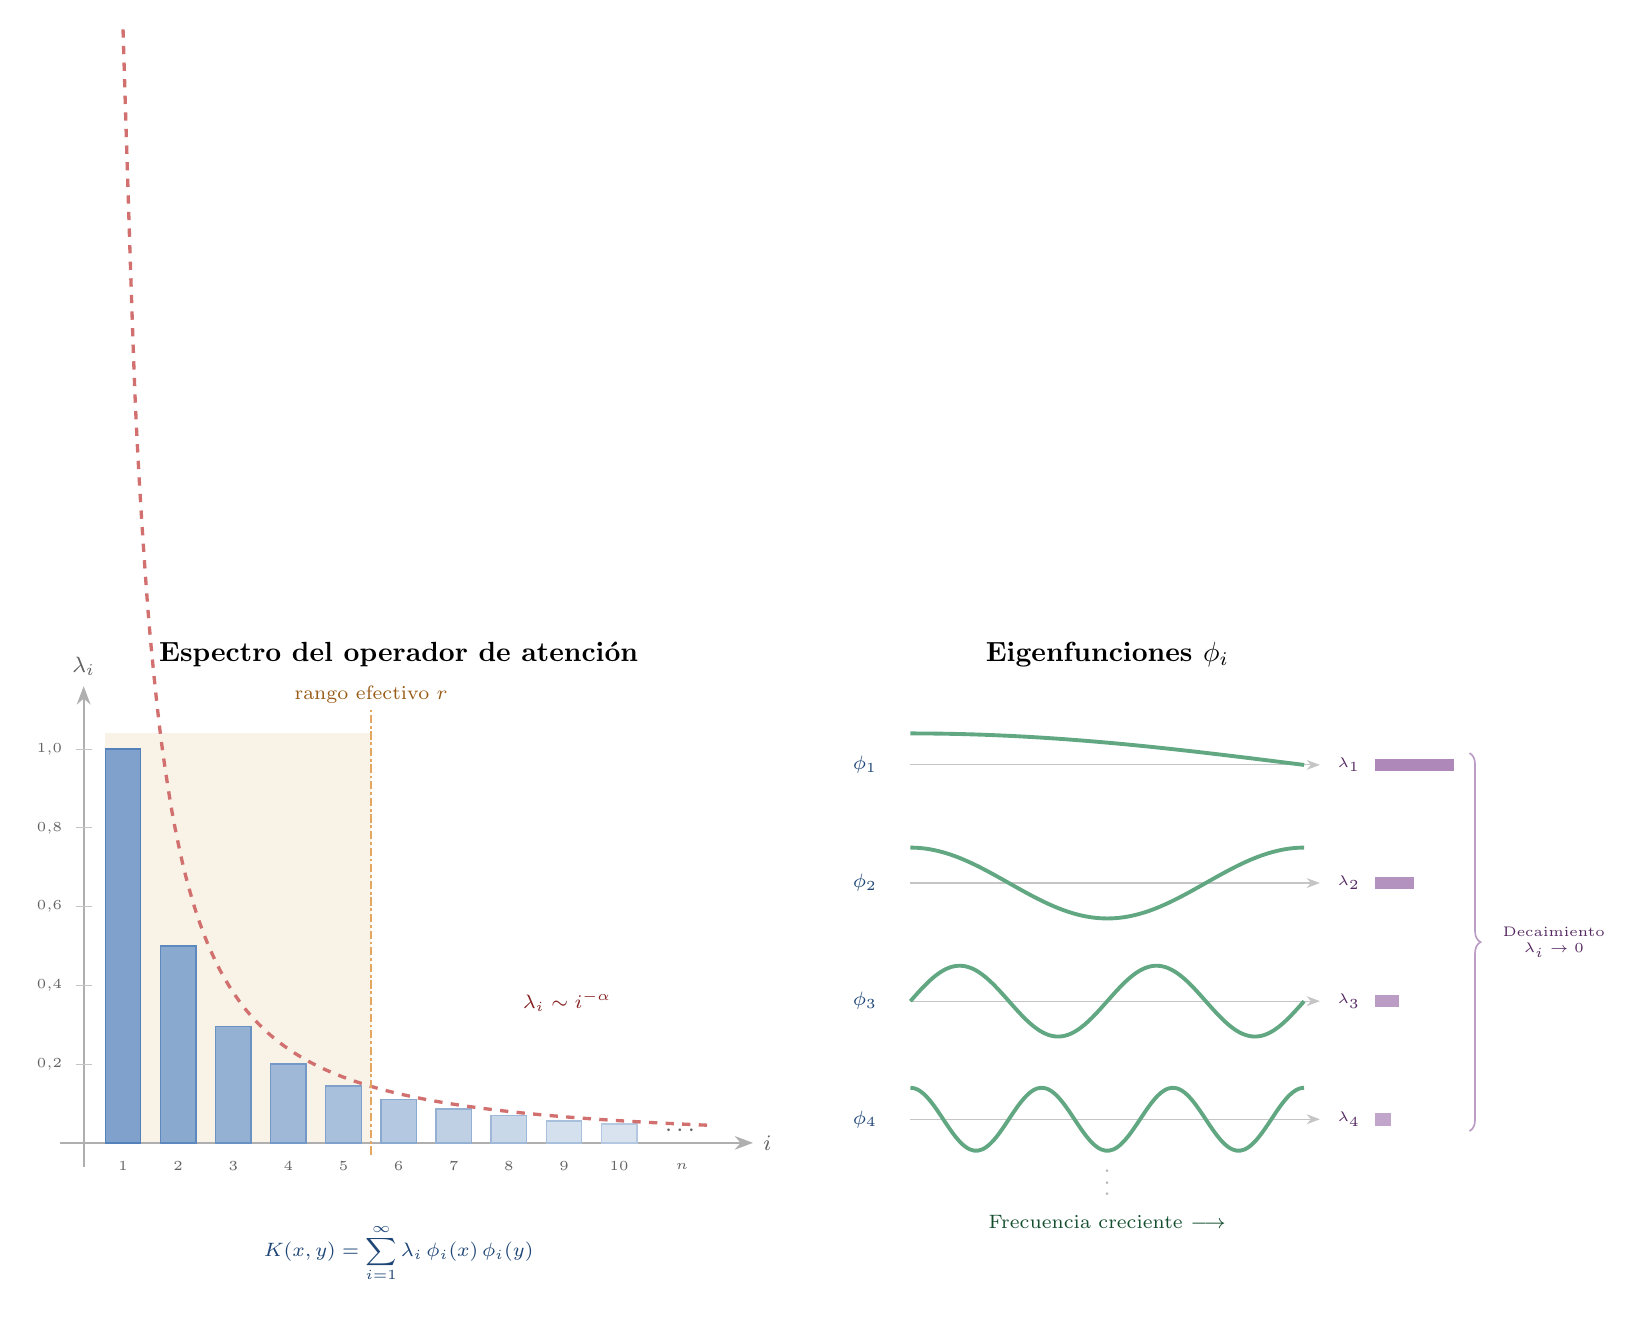
\begin{tikzpicture}[>=Stealth, font=\small]

% ============================================================
% LEFT PANEL: Eigenvalue spectrum (bar chart)
% ============================================================
\begin{scope}[shift={(0,0)}]

  % Title
  \node[font=\bfseries, text=black] at (4.0, 6.2)
    {Espectro del operador de atenci\'{o}n};

  % Shade the "significant" region (draw first, behind bars)
  \fill[gdlyellow!10] (0.27, 0) rectangle (3.65, 5.2);

  % Axes
  \draw[->, gdlgray!70, line width=0.8pt] (-0.3, 0) -- (8.5, 0)
    node[right, font=\footnotesize, text=gdlgray!70!black] {$i$};
  \draw[->, gdlgray!70, line width=0.8pt] (0, -0.3) -- (0, 5.8)
    node[above, font=\footnotesize, text=gdlgray!70!black] {$\lambda_i$};

  % Y-axis ticks
  \foreach \y/\lab in {1/0{,}2, 2/0{,}4, 3/0{,}6, 4/0{,}8, 5/1{,}0} {
    \draw[gdlgray!50] (-0.1, \y) -- (0.1, \y);
    \node[font=\tiny, text=gdlgray!70!black, anchor=east] at (-0.15, \y) {$\lab$};
  }

  % Eigenvalue bars with rapid decay
  \def\barwidth{0.45}

  \fill[gdlblue!60] (0.5-\barwidth/2, 0) rectangle (0.5+\barwidth/2, 5.0);
  \draw[gdlblue!80, line width=0.5pt] (0.5-\barwidth/2, 0) rectangle (0.5+\barwidth/2, 5.0);
  \node[font=\tiny, text=gdlgray!70!black] at (0.5, -0.3) {$1$};

  \fill[gdlblue!55] (1.2-\barwidth/2, 0) rectangle (1.2+\barwidth/2, 2.5);
  \draw[gdlblue!75, line width=0.5pt] (1.2-\barwidth/2, 0) rectangle (1.2+\barwidth/2, 2.5);
  \node[font=\tiny, text=gdlgray!70!black] at (1.2, -0.3) {$2$};

  \fill[gdlblue!50] (1.9-\barwidth/2, 0) rectangle (1.9+\barwidth/2, 1.48);
  \draw[gdlblue!70, line width=0.5pt] (1.9-\barwidth/2, 0) rectangle (1.9+\barwidth/2, 1.48);
  \node[font=\tiny, text=gdlgray!70!black] at (1.9, -0.3) {$3$};

  \fill[gdlblue!45] (2.6-\barwidth/2, 0) rectangle (2.6+\barwidth/2, 1.0);
  \draw[gdlblue!65, line width=0.5pt] (2.6-\barwidth/2, 0) rectangle (2.6+\barwidth/2, 1.0);
  \node[font=\tiny, text=gdlgray!70!black] at (2.6, -0.3) {$4$};

  \fill[gdlblue!40] (3.3-\barwidth/2, 0) rectangle (3.3+\barwidth/2, 0.72);
  \draw[gdlblue!60, line width=0.5pt] (3.3-\barwidth/2, 0) rectangle (3.3+\barwidth/2, 0.72);
  \node[font=\tiny, text=gdlgray!70!black] at (3.3, -0.3) {$5$};

  \fill[gdlblue!35] (4.0-\barwidth/2, 0) rectangle (4.0+\barwidth/2, 0.55);
  \draw[gdlblue!55, line width=0.5pt] (4.0-\barwidth/2, 0) rectangle (4.0+\barwidth/2, 0.55);
  \node[font=\tiny, text=gdlgray!70!black] at (4.0, -0.3) {$6$};

  \fill[gdlblue!30] (4.7-\barwidth/2, 0) rectangle (4.7+\barwidth/2, 0.43);
  \draw[gdlblue!50, line width=0.5pt] (4.7-\barwidth/2, 0) rectangle (4.7+\barwidth/2, 0.43);
  \node[font=\tiny, text=gdlgray!70!black] at (4.7, -0.3) {$7$};

  \fill[gdlblue!25] (5.4-\barwidth/2, 0) rectangle (5.4+\barwidth/2, 0.35);
  \draw[gdlblue!45, line width=0.5pt] (5.4-\barwidth/2, 0) rectangle (5.4+\barwidth/2, 0.35);
  \node[font=\tiny, text=gdlgray!70!black] at (5.4, -0.3) {$8$};

  \fill[gdlblue!20] (6.1-\barwidth/2, 0) rectangle (6.1+\barwidth/2, 0.28);
  \draw[gdlblue!40, line width=0.5pt] (6.1-\barwidth/2, 0) rectangle (6.1+\barwidth/2, 0.28);
  \node[font=\tiny, text=gdlgray!70!black] at (6.1, -0.3) {$9$};

  \fill[gdlblue!18] (6.8-\barwidth/2, 0) rectangle (6.8+\barwidth/2, 0.24);
  \draw[gdlblue!35, line width=0.5pt] (6.8-\barwidth/2, 0) rectangle (6.8+\barwidth/2, 0.24);
  \node[font=\tiny, text=gdlgray!70!black] at (6.8, -0.3) {$10$};

  % Dots for continuation
  \node[font=\small, text=gdlgray!70!black] at (7.6, 0.15) {$\cdots$};
  \node[font=\tiny, text=gdlgray!70!black] at (7.6, -0.3) {$n$};

  % Decay envelope curve
  \draw[gdlred!70, line width=1.2pt, dashed, smooth]
    plot[domain=0.5:8.0, samples=50] (\x, {5.0/(\x)^1.5});

  % Label for decay
  \node[font=\scriptsize, text=gdlred!70!black, anchor=west, fill=white,
        fill opacity=0.85, text opacity=1, inner sep=2pt, rounded corners=1pt]
    at (5.5, 1.8) {$\lambda_i \sim i^{-\alpha}$};

  % Effective rank cutoff line
  \draw[gdlorange!70, line width=1.0pt, densely dash dot]
    (3.65, -0.15) -- (3.65, 5.5);
  \node[font=\scriptsize, text=gdlorange!70!black, anchor=south, fill=white,
        fill opacity=0.85, text opacity=1, inner sep=2pt, rounded corners=1pt]
    at (3.65, 5.5) {rango efectivo $r$};

  % Mercer formula
  \node[font=\scriptsize, text=gdlblue!70!black, align=center, anchor=north]
    at (4.0, -0.9)
    {$K(x,y) = \displaystyle\sum_{i=1}^{\infty} \lambda_i \,\phi_i(x)\,\phi_i(y)$};

\end{scope}

% ============================================================
% RIGHT PANEL: Eigenfunctions (harmonic patterns)
% ============================================================
\begin{scope}[shift={(10.5, 0)}]

  % Title
  \node[font=\bfseries, text=black] at (2.5, 6.2)
    {Eigenfunciones $\phi_i$};

  % --- phi_1: nearly constant (fundamental mode) ---
  \node[font=\scriptsize, text=gdlblue!70!black, anchor=east] at (-0.3, 4.8)
    {$\phi_1$};
  \draw[->, gdlgray!50, line width=0.4pt] (0, 4.8) -- (5.2, 4.8);
  \draw[gdlgreen!70, line width=1.4pt, smooth]
    plot[domain=0:5, samples=40] (\x, {4.8 + 0.4*cos(18*\x)});
  % eigenvalue bar
  \node[font=\tiny, text=gdlpurple!70!black, anchor=west] at (5.3, 4.8) {$\lambda_1$};
  \fill[gdlpurple!60] (5.9, 4.72) rectangle (6.9, 4.88);

  % --- phi_2: one oscillation (first harmonic) ---
  \node[font=\scriptsize, text=gdlblue!70!black, anchor=east] at (-0.3, 3.3)
    {$\phi_2$};
  \draw[->, gdlgray!50, line width=0.4pt] (0, 3.3) -- (5.2, 3.3);
  \draw[gdlgreen!70, line width=1.4pt, smooth]
    plot[domain=0:5, samples=60] (\x, {3.3 + 0.45*cos(72*\x)});
  \node[font=\tiny, text=gdlpurple!70!black, anchor=west] at (5.3, 3.3) {$\lambda_2$};
  \fill[gdlpurple!55] (5.9, 3.22) rectangle (6.4, 3.38);

  % --- phi_3: two oscillations (second harmonic) ---
  \node[font=\scriptsize, text=gdlblue!70!black, anchor=east] at (-0.3, 1.8)
    {$\phi_3$};
  \draw[->, gdlgray!50, line width=0.4pt] (0, 1.8) -- (5.2, 1.8);
  \draw[gdlgreen!70, line width=1.4pt, smooth]
    plot[domain=0:5, samples=80] (\x, {1.8 + 0.45*sin(144*\x)});
  \node[font=\tiny, text=gdlpurple!70!black, anchor=west] at (5.3, 1.8) {$\lambda_3$};
  \fill[gdlpurple!50] (5.9, 1.72) rectangle (6.2, 1.88);

  % --- phi_4: three oscillations (third harmonic) ---
  \node[font=\scriptsize, text=gdlblue!70!black, anchor=east] at (-0.3, 0.3)
    {$\phi_4$};
  \draw[->, gdlgray!50, line width=0.4pt] (0, 0.3) -- (5.2, 0.3);
  \draw[gdlgreen!70, line width=1.4pt, smooth]
    plot[domain=0:5, samples=100] (\x, {0.3 + 0.4*cos(216*\x)});
  \node[font=\tiny, text=gdlpurple!70!black, anchor=west] at (5.3, 0.3) {$\lambda_4$};
  \fill[gdlpurple!45] (5.9, 0.22) rectangle (6.1, 0.38);

  % Vertical dots
  \node[font=\small, text=gdlgray!60] at (2.5, -0.4) {$\vdots$};

  % Annotation: frequency interpretation
  \node[font=\scriptsize, text=gdlgreen!60!black, align=center, anchor=north]
    at (2.5, -0.8)
    {Frecuencia creciente $\longrightarrow$};

  % Bracket for eigenvalue bars
  \draw[gdlpurple!50, line width=0.6pt, decorate,
        decoration={brace, amplitude=4pt, mirror}]
    (7.1, 0.15) -- (7.1, 4.95);
  \node[font=\tiny, text=gdlpurple!70!black, anchor=west, align=center] at (7.4, 2.55)
    {Decaimiento\\$\lambda_i \to 0$};

\end{scope}

\end{tikzpicture}
\end{document}
